The system that is described in this section is currently in pilot phase and is planned to \emph{replace} the infrastructure of section \ref{sec-phys-infra} in Q2 2021.

The physical servers are replaced with a cluster of virtual machines composing an Openshift Kubernetes (OKD 4.6) cluster.
Openshift is a Kubernetes distribution that extends vanilla Kubernetes with additional APIs and comes bundled with preconfigured components for infrastructure functionality:
UI friendly to the end users, standardized multitenancy and ingress controllers, Prometheus
% TODO rajula
% Add sophisticated description of Openshift

Instead of the Apache vhost and a part of the PHP-FPM pool, each website is served by 1 or multiple replicas of a pod,
with an Nginx and PHP-FPM containers.
The journey of an HTTP request through the new infrastructure, shown in figure \ref{fig:drupal-physical-request-journey},
holds a strong analogy to the journey through the physical infrastructure in figure \ref{fig:drupal-physical-request-journey}.

\begin{figure}[ht]
    \centering
    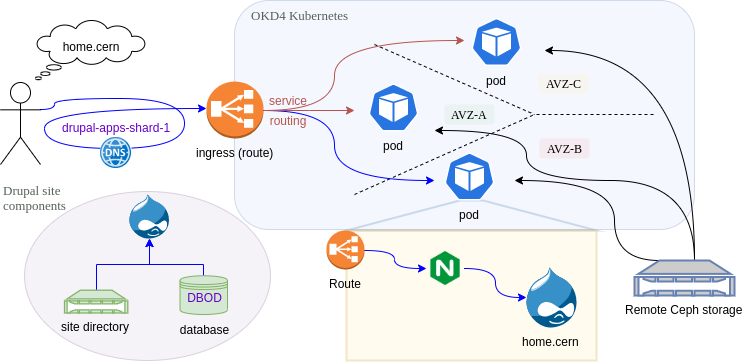
\includegraphics[width=\textwidth]{figures/drupal-k8s-request-journey}
    \caption{Caption}
    \label{fig:drupal-k8s-request-journey}
\end{figure}

\subsubsection*{Website management functions}

The infrastructure can be seen as an application that offers its users functions to manage websites.
It provides an API for website admins to specify the kind of website they need: what version of Drupal, what amount of resources, which git repository to fetch configuration from.
Website admins should similarly be able to create new environments of their website for development or test purposes,
clone data between websites, and take and restore backups.

CMS-based websites are inherently stateful applications: end users interact with them constantly and progress their state,
which is stored in a database and in a persistent volume.
To facilitate development, the state of a Drupal application can be "cloned" into another Drupal website.
The development workflow includes ... % TODO

\subsection{Operator pattern}

The design of the management application hinges on Kubernetes controllers and APIs.


\subsection{System components}

\begin{figure}[ht]
    \centering
    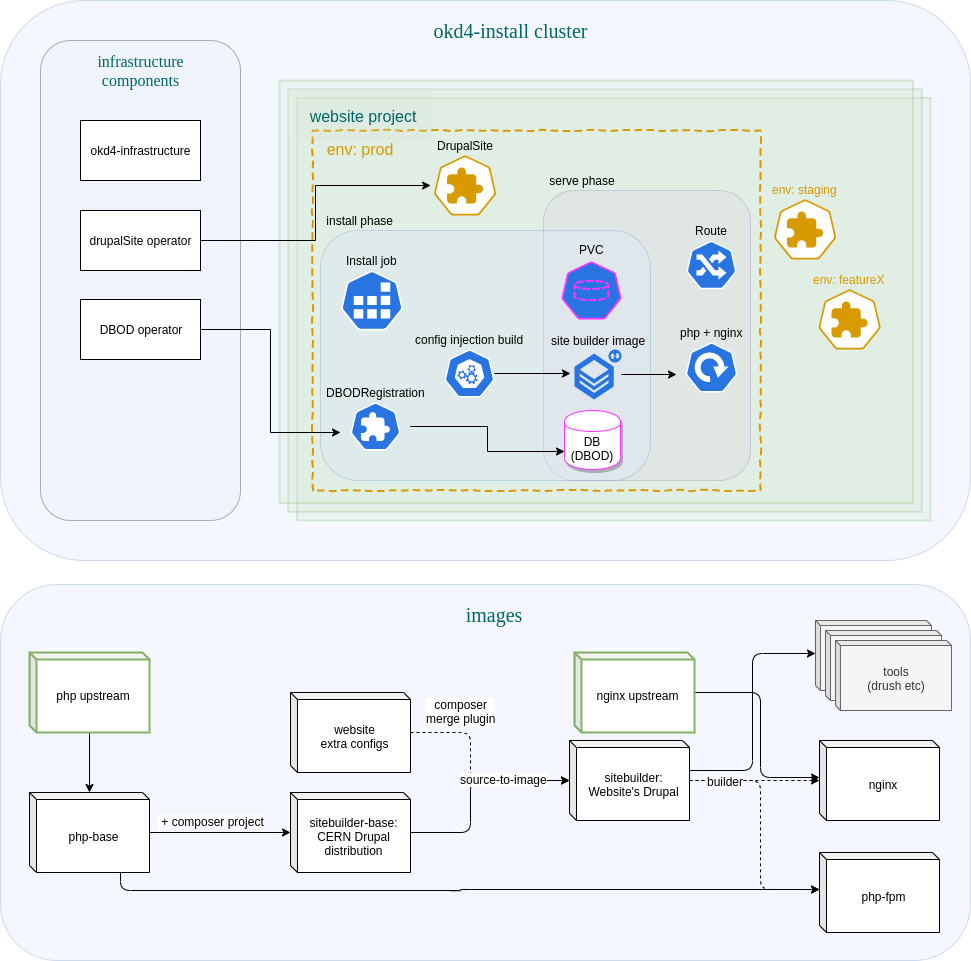
\includegraphics[width=\textwidth]{figures/drupal-k8s-architecture}
    \caption{Caption}
    \label{fig:my_label}
\end{figure}


%%% NOTES %%%

diagrams
- [x] serve request journey
- [v] architecture
- admin workflow to update Drupal version
- build configs / auto triggers (maybe merge above)

% TODO
Analyse the "okd4-infrastructure" components.
Describe the authz-operator, custom ingress, cephfs, velero.

%/subsection{Operator pattern}

https://www.openshift.com/learn/topics/operators

Kubernetes design principles, operators


L7 cloud load balancing for .cern domains?